% Created 2018-11-07 Wed 23:46
% Intended LaTeX compiler: pdflatex
\documentclass[11pt]{article}
\usepackage[utf8]{inputenc}
\usepackage[T1]{fontenc}
\usepackage{graphicx}
\usepackage{grffile}
\usepackage{longtable}
\usepackage{wrapfig}
\usepackage{rotating}
\usepackage[normalem]{ulem}
\usepackage{amsmath}
\usepackage{textcomp}
\usepackage{amssymb}
\usepackage{capt-of}
\usepackage{hyperref}
\usepackage[toc,acronyms]{glossaries}
\usepackage[round]{natbib}
\usepackage{svg}
\usepackage{array}
\makeglossaries
\newcommand\blfootnote[1]{\begingroup\renewcommand\thefootnote{}\footnote{#1}\addtocounter{footnote}{-1}\endgroup}
\usepackage{subcaption}
\newcolumntype{L}[1]{>{\raggedright\let\newline\\\arraybackslash\hspace{0pt}}m{#1}}
\newacronym{ai}{AI}{Artificial Intelligence}
\newacronym{aida}{AIDA}{Artificial Intelligence Development Act}
\newacronym{ubc}{UBC}{University of British Columbia}
\newacronym{nn}{NN}{neural network}
\newacronym{sa}{SA}{sentiment analysis}
\newacronym{nstc}{NSTC}{National Science and Technology Council}
\newacronym{rd}{R\&D}{research and development}
\newacronym{mlai}{MLAI}{machine learning and artificial intelligence}
\author{Jasper}
\date{\today}
\title{Ethics of Artificial Intelligence in the North-American Workplace}
\hypersetup{
 pdfauthor={Jasper},
 pdftitle={Ethics of Artificial Intelligence in the North-American Workplace},
 pdfkeywords={},
 pdfsubject={},
 pdfcreator={Emacs 26.1 (Org mode 9.1.9)}, 
 pdflang={English}}
\begin{document}

\maketitle
\tableofcontents

\listoftables
\listoffigures

\glsaddall \printglossary[type=\acronymtype]


\begin{abstract}
\gls{ai} is becoming increasingly prominent in the workplace, with systems appearing everywhere from smartphones to cars. 
With this increase of \gls{ai} systems, more ethical issues regarding their usage are becoming apparent. 
\gls{ai} systems are are incredibly complicated and often considered “black boxes” due to the lack of understanding and trust society has with regards to their inner workings. 
The use of neural networks and data testing using known inputs and outputs, pose the challenge of verifying whether \gls{ai} is suitable for a task. 
Using AI in daily life demands significant  human computer interaction, which means that any biases inherent to \gls{ai} will propagate to human interaction. 
These biases, usually the result of impressionable programming, data acquisition, and machine learning, are detrimental to workplace accessibility and equality. 
When \gls{ai} makes mistakes, the question of liability and accountability arises. 
Two options exist for holding accountability: the \gls{ai} system, and creator. 
Due to these ethical issues, guidelines must be created and observed by both users and creators. 
Organizations have already begun recommending \gls{ai} guidelines following humanitarian law for a more ethical use of \gls{ai}. 
Unless these issues are acknowledged, they risk multiplying as \gls{ai} manages more responsibility and riskier tasks in the future. 
\end{abstract}

\section{Introduction}
\label{sec:orgff7efbb}
The notion of artificial intelligence has long been associated with progress and prosperity. 
Yet its recent emergence in modern life may not prove as much. 
The influx of artificial intelligence uses in the North-American workplace has introduced various ethical dilemmas. 
Specifically, it has reshaped communication to necessitate less and less human interaction by augmenting human-computer interaction. 
Despite the various advantages to automation, the ethical concerns it raises call into question its appropriate extent in the workplace, and beyond. 
Based on information collected from reputable sources made available through \gls{ubc}’s library databases, the main ethical concerns have been identified. 
The transparency, bias, accountability,and regulation of \gls{ai} are being examined. 

\section{Allocation of Accountability}
\label{sec:org31c733a}
\subsection{Assessing Responsibility}
\label{sec:orgd858497}
With the noticeable increase of \gls{ai} use in the workplace and potential institutional dependency on it, several concerns arise. 
While \gls{ai} functions by analyzing its surroundings, generating alternatives and finding the best outcome it deems possible, \gls{ai} ethical decision making remains questionable by humans. 
As such, it is crucial to address the question: who is held accountable for risks arising from \gls{ai} decision making? 

\gls{ai} accountability can be assessed through two approaches. 
The first approach, the classic approach, views machines as slaves or mechanical instruments controlled and owned by humans, thus bearing no responsibility. 
The second approach, the pragmatic approach, on the other hand, holds \gls{ai} accountable for their actions and decisions under the coat of `artificial morality' \citep{alaieri2016}.
This, however, is dependent on how the \gls{ai} was programmed initially. 
If the \gls{ai} was programmed using the the `top-down' method, where ethical codes are embedded by the programmer, then the coder is fully responsible for the actions for his or her \gls{ai}. 
There may be inherent problems with this approach, Liu notes ``guiding ethical frameworks overlook compound or aggregated effects which may arise, and which can lead to subtle forms of structural discrimination\citep[p.1]{liu2017}.
But if the \gls{ai} was coded using the `bottom up' method, where \gls{ai} is able to learn for its surrounding and learn from experience, then the \gls{ai} is fully responsible of its actions. 
The \gls{ai}, its manufacturers as well as its users can all be held accountable for any negative outcomes resulting from the \gls{ai}. 

There are many use cases for \gls{ai}, particularly in the case of user error or unscrupulous behaviour by users, \gls{ai} outcomes can be undesirable. 
In such cases, of course, the user would be responsible for any outcomes. 
For example, the Microsoft's Twitter chatbot was noticed to be tweeting sexist and racist responses. 
This is due to the fact that the intelligence improved through experiential learning, Twitter users having learnt this, intentionally made sexist and racist comments in an effort to impact its decisions \citep{alaieri2016}.

\subsection{Applications and Practice}
\label{sec:orgef3d8d1}
\gls{ai} is arguably better at `rational' decision making than humans but the lack of human trust in \gls{ai} decision making sustains a fear of negative outcomes.
\gls{ai} will give the output without any further explanation, even if the decision making process is opaque. 
This means that in some cases \gls{ai} makes the `rational' response but human perception may not reach the same conclusion and hence think the decision made by the \gls{ai} was unethical \citep{alaieri2016}.

Thus for a more practical way of allocating accountability, it is suggested that a certifying agency be created under the purview of the \Gls{aida} that evaluates the safety of \gls{ai}. 
If manufacturers pass the certificate, then they would hold limited liability of whatever the outcomes of their \gls{ai} produces, however, if an \gls{ai} product isn't `certified' then the producer/programmer is to be hold responsible for the negative or unethical decisions made by their \gls{ai} \citep{scherer2016}.
The accountability of \gls{ai} thus, depends on multiple factors and differs when looked at from multiple perspectives. 
This indicates that more work should be put onto the regulations of the use of \gls{ai} to resolve the ethical concerns of its decision making in the workplace. 

\section{Unintentional Bias of \acrshort{ai}}
\label{sec:orgf3f1c5c}
The notion that \gls{ai} can be objective is an attractive prospect. 
Using \gls{ai} in lieu of a human could serve in eliminating any preconceptions or judgements that are unrelated to the task at hand. 
This symbolizes an advantageous elimination of unethical treatment in the workplace, and beyond. 
However, much like the people that make them, \gls{ai} can equally be riddled with biases. 
The plausibility of a truly bias free \gls{ai} is under question. 

\begin{figure}[htbp]
\centering
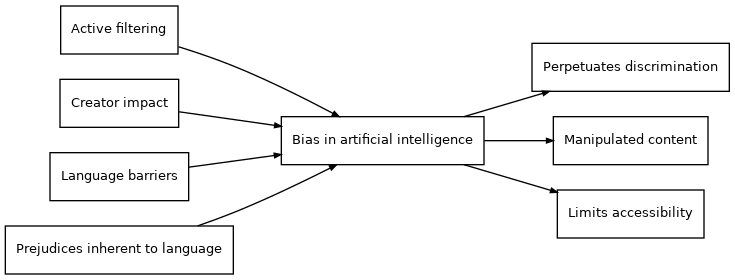
\includegraphics[width=.9\linewidth]{constituents.png}
\caption[Constituents and Effects of \gls{ai} Biases]{The Constituents and Potential Effects of \gls{ai} Biases. \label{fig-constituents}}
\end{figure}

\subsection{Prejudice and Accessibility}
\label{sec:org53d09f9}
With the ever-increasing presence of \gls{ai} in the workplace, interactions with this technology become more significant.
It is a powerful tool, but it can equally be detrimental.
\gls{ai} parameters may decrease accessibility and perpetuate stereotypes by the means illustrated in Figure \ref{fig-constituents}.

A popular use of \gls{ai} consists of virtual personal assistants, such as Apple's Siri or Microsoft's Cortana. 
Yet their use is not available to all. 
Voice automated technologies often fall short when it comes to recognizing various dialects or non-standardized speech \citep{hirayama2015}. 
This bars people with such manners of speech from using a helpful technology that facilitates work. 

Human interaction with \gls{ai} involves a heavy amount of filtering. 
It is often used to better suit a user's needs. 
Yet it can also serve as a method of advertisement and withhold useful information. 
The bias in the filtering process is a product of personalized algorithms, the influence of the creator, and intentional content selection by the technology's owner \citep{bozdag2013}. 
This can limit \gls{ai}'s flexibility and range in informational output, providing the user partial results.

The characterization of biases within \gls{ai} is inexact and the bestowment of the title is often contested. 
Nonetheless, there exists biases in \gls{ai} that are undeniable biases. Sexism, racism, and the likes are ethical dilemmas to which \gls{ai} are susceptible. 
The documented instances of racial prejudice in \gls{ai} \citep{danks2017} risk perpetuating harmful stereotypes and racism. 

\begin{table}[htbp]
\caption[Word Vector Associations with "She" and "He"]{The Strongest Word Vector Associations with "She" and "He" found in Word2Vec \footnotemark. Created with data from \cite{bolukbasi2016} \label{tbl-wordvec}}
\centering
\begin{tabular}{c|c}
She & He\\
\hline
Homemaker & Maestro\\
Nurse & Protégé\\
Receptionist & Philosopher\\
Librarian & Captain\\
Socialite & Architect\\
Hairdresser & Financer\\
Nanny & Warrior\\
\end{tabular}
\end{table}

\(\footnotetext{Word2Vec is a complex embedding created on a corpus of Google News with 3 million words \citep{bolukbasi2016}.}\)

Methods of machine learning, such as semantics achieved through word embedding\footnote{Word-embedding is the mathematical representation of conceptual associations within language} , are liable to precisely reflect the biases seen in humans \citep{caliskan2017}. 
This compromises any hope of objectivity and holds ethical ramifications. 

For example, Bryson, Caliskan, and Narayanan noted how the word "she" was associated with words pertaining to domestic roles, examples of these associations are available in Table \ref{tbl-wordvec}. 
This is counteractive to the sociopolitical progress made by women. 
It compromises women’s and minorities’ importance and personal development within the workplace. 

\subsection{The Search for Objectivity}
\label{sec:org0e7fe8f}
Some argue that unbiased \gls{ai} is likely unachievable \citep{bozdag2013}. 
Any product of humans is prone to echo their same partiality. 
Nevertheless, the mitigation of some detrimental biases is possible. 
Speech recognition in \gls{ai} has been improved upon to respond to a wider array of dialects \citep{hirayama2015}, increasing accessibility. Biases are arguably an inherent part of the algorithms on which \gls{ai} is based \citep{danks2017}. 
The solution may lie in bias mitigation at the source: humans.

\section{Transparency in \acrshort{ai} Decision Making}
\label{sec:org8ca1baa}
Being still an emerging technology, truly autonomous \gls{ai} is still far from being a reality.
There are still many problems that must be solved before \gls{ai} can be used safely and ethically.

\subsection{Overview of Neural Network Based Systems}
\label{sec:org54f3627}
A \Gls{nn} can simply be thought of as a function that takes inputs and produces some output. 
For example, a \gls{nn} that classifies numbers might take pictures of handwritten digits as inputs. 

\begin{figure}
\begin{center}
\begin{subfigure}[t]{.15\textwidth}
\begin{center}

\includegraphics[width=1.5cm]{0.jpg}
\end{center}
\caption*{label=5}
\end{subfigure}
\begin{subfigure}[t]{.15\textwidth}
\begin{center}

\includegraphics[width=1.5cm]{1.jpg}
\end{center}
\caption*{label=0}
\end{subfigure}
\begin{subfigure}[t]{.15\textwidth}
\begin{center}

\includegraphics[width=1.5cm]{2.jpg}
\end{center}
\caption*{label=4}
\end{subfigure}
\begin{subfigure}[t]{.15\textwidth}
\begin{center}

\includegraphics[width=1.5cm]{3.jpg}
\end{center}
\caption*{label=1}
\end{subfigure}
\begin{subfigure}[t]{.15\textwidth}
\begin{center}

\includegraphics[width=1.5cm]{4.jpg}
\end{center}
\caption*{label=9}
\end{subfigure}
\end{center}
\caption[Handwritten Digit Samples]{Images of handwritten digits and their labels from the MNIST database \citep{mnistdb} \label{fig-mnist_digits}}
\end{figure}


The input layer would have one neuron per pixel in the image, with the activation being the pixel's brightness.
The output layer would one neuron for each digit.
In between these layers are what are called ``hidden layers''.
Each neuron in a layer are connected to every neuron from the previous layer.
Each of these connections will have some unique weight that represents how strongly correlated they are.


\begin{figure}[htbp]
\centering
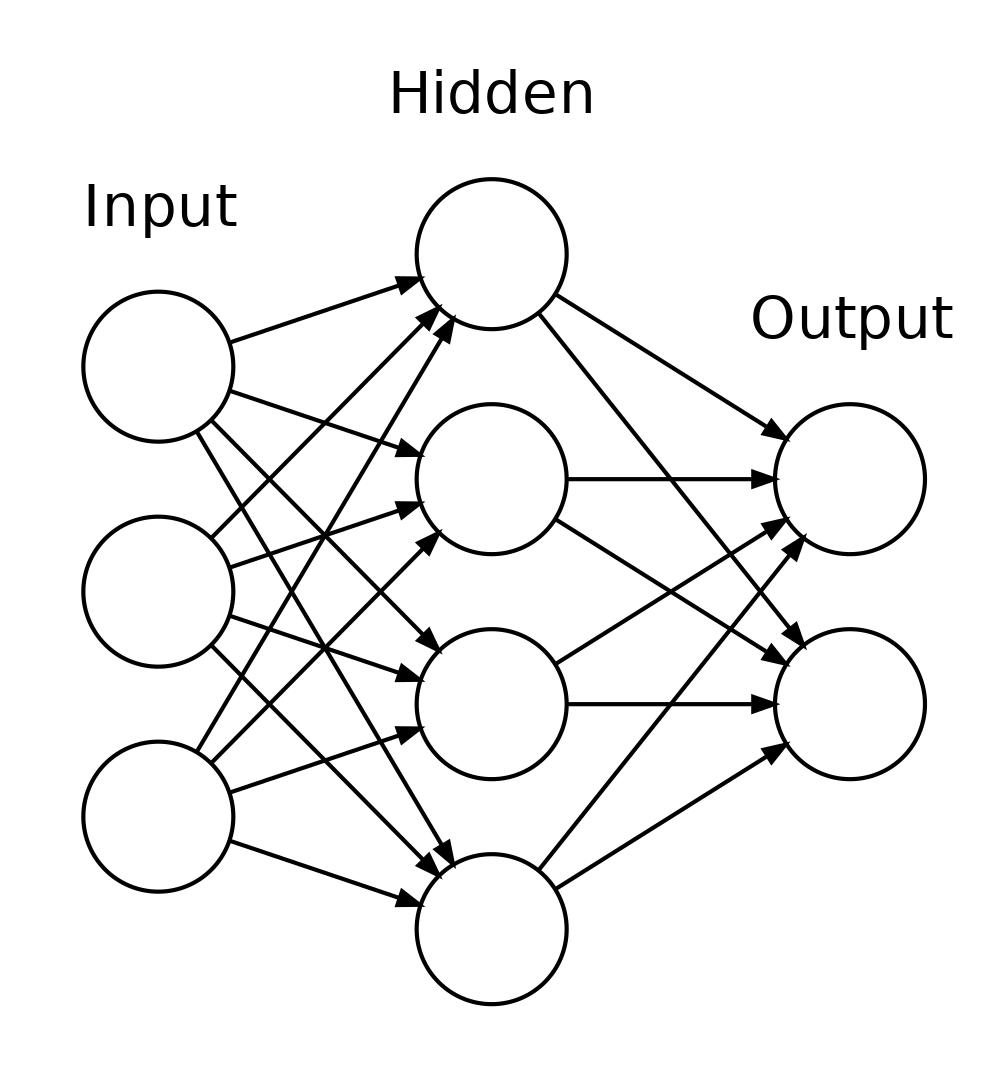
\includegraphics[width=.9\linewidth]{nn.png}
\caption[Visual Representation of a Neural Network]{A visual representation of a small neural network with 3 inputs, 2 outputs, and one hidden layer. \label{fig-nn}}
\end{figure}


The activation of a given neuron is then calculated as follows:
\begin{equation}\label{eqn:activation}
	a_{(i,j)} = \sigma \left( \left( \sum\limits_{n=1}^N = a_{(n,j-1)}w_{(n,j-1)|(i,j)} \right) + b_{(i,j)} \right)
\end{equation}
\(\blfootnote{Equation (\ref{eqn:activation}) describes the summing of the activation of all of the previous neurons plus some bias, and then normalizing it using the sigmoid function.}\)

The weights are calculated for every neuron until they reach the output layer, where they hopefully give meaningful output.
Here, a good output would be the neuron representing the correct digit having high activation, while the other neurons have low activation.

\subsection{Using Training Data in the Real World}
\label{sec:orgfff31c1}
When a \gls{nn} is created, the weights are unset and the network produces random noise for any given input.
To make the network produce meaningful data it must be trained.
Training is done by providing input, comparing its output to the expected output, and adjusting the weights accordingly\footnote{This is done with back-propagation, which essentially means adjusting the weights between the final layers, then adjusting the ones before that, until all the layers have been adjusted.}.

One of the problems that arises from this is that the \gls{nn} becomes optimized for the training data.
Because of this, it is not guaranteed to perform well on a different set of data \citep{amodei2016}. 
While this problem is not specific to \gls{ai} \footnote{i.e. an untrained human will also be poor at the same task}, \glspl{nn} are unable to recognize that they are untrained.
This could create ethical issues when creating \gls{ai} that must communicate to a user.
By being trained on data from one cultural region, the \gls{ai} may lack cultural awareness of others.



\subsection{Current and Future Ethical Implications of Using \acrshort{ai} in the Workplace}
\label{sec:orgf69f2bb}
One of the applications of \gls{ai} is \Gls{sa}.
\gls{sa} is used to identify someone's attitude towards some topic.
Predictably, this technology has become highly sought after by businesses \citep{alexandra2014}.
\Gls{sa} can be used to read the publics' reaction to something, or provide information for optimizing marketing campaigns.
However, it can also be used to monitor an employee's communications.
This could have serious ethical implications since it would be impossible for an employee to know what messages may get flagged.
An employee could be fired without ever saying something against company policy.

As \gls{ai} systems become more general, they will replace humans in more and more areas.
It is imperative that these \gls{ai} systems act in an ethical manner.
One of the most important things to consider is how to define an \gls{ai}'s goals.
For example, a general \gls{ai} may be self-protective so that it may continue to achieve its goal \citep{omohundro2014}, leading to unwanted behavior.
Because of the opaque nature of \gls{ai}, it will be hard to verify that a given system completely follows its intended purpose.

\section{Guidelines for \acrshort{ai} Usage}
\label{sec:org6065c4d}
To address the issues with \gls{ai}, guidelines must be created and observed by producers and users.
Creating guidelines for \gls{ai} is difficult, but crucial to address the downfalls of \gls{ai}.

\subsection{Creating Guidelines for the Future}
\label{sec:org0fdfead}
Many organizations have already begun looking at the effects of \gls{ai} on the future society.
The One-Hundred-Year Study On \gls{ai} from Stanford University outlines some aspects required to create effective guidelines: 
Place experts who understand \gls{ai} interaction in government in order to property evaluate \gls{ai} impact and recommend a path of action; 
Fund interdisciplinary studies to look at the social impact of \gls{ai}; 
and, remove impediments to allow research on fairness and security of \gls{ai} which is critical for examining accountability for \gls{ai} systems \citep{stone2016}.
Creating guidelines will take time and a lot work is still needed, yet the first steps were already taken by the white house last year as two reports outlining a strategy for \gls{ai} \Gls{rd} were published.
The \Gls{nstc} \Gls{mlai} community outlined over twenty recommendations, some major ones are presented in Table \ref{tbl-ntscrec} below \citep{nstc2016}.

\begin{table}[htbp]
\caption{Key \gls{nstc} Recommendations \label{tbl-ntscrec}}
\centering
\begin{tabular}{l|L{5in}}
\gls{nstc} Number & Recommendation\\
\hline
1 & Institutions should examine whether and how they can responsibly use \gls{mlai}\\
2 & Federal agencies should prioritize open data training and open data standards in \gls{ai}\\
4 & The \gls{nstc} \gls{mlai} subcomittee should develop a group for \gls{ai} practitioners across government\\
11 & The government should monitor the milestones of \gls{ai} development in other countries\\
13 & The federal government should prioritize short and long-term \gls{ai} \gls{rd}\\
18 & Schools should include ethics, and discussions about security, privacy, and safety, as part of a curricula on \gls{ai}, and machine learning\\
20 & The government should develop a strategy on international engagement, and a list of \gls{ai} areas that need international engagement and monitoring\\
23 & The government should finish developing of a single policy, consistent with humanitarian law, on autonomous and semi-autonomous weapons\\
\end{tabular}
\end{table}


As a budding topic, \gls{ai} is becoming more prominent and concerns are being raised on how it will change the society.
A concern for many people is losing their jobs to automation. 
Moreover, the development of \gls{ai} will cause inequality and greater bias in the labour market as low-skilled jobs disappear creating way for more high-skilled jobs \citep{leenes2017}.
Therefore, this issue, like many other, must be addressed in the future guidelines, but including all ethical issues is difficult.

\subsection{The Challenge of Creating Guidelines}
\label{sec:orgb872086}
The major challenge of creating regulation for \gls{ai} is keeping up with the technological advances. 
Since \gls{ai} technology is new and evolving, there will be gaps in existing regulation and new laws to be made to adapt to the technology. 
However, since the technology is advancing rapidly more conflicts will arise with existing regulations. 
This dilemma for controlling evolving technology is called technology-neutrality versus legal certainty. 
One method is controlling the effects of \gls{ai} using abstract regulations that can apply to many cases, yet this may not provide enough legal constraints and certainty. 
On the other hand, having strong legal certainty and premature laws may obstruct the scientific advancement and stop innovation. 
Legal regulations can’t be adapted to include new advancing technology or use reclassification to include evolving technology in an existing distinction, new neutral and legal constrained need to be created \citep{leenes2017}. 

Regulating \gls{ai} comes with the challenge of following ethical standards, and a strong value system of overarching principles. 
The issue of accountability must be addressed in the legal regulations, transparent research must be conducted to allow clear future guidelines for \gls{ai} use, and biases must be considered in order to decide whether \gls{ai} would strengthen existing bias or create new biases. 
The ethical principles should be key part in the creation of new guidelines but also impose the big challenge on the creation of proper guidelines. 

\section{Conclusion}
\label{sec:orgc4fccb6}
It is undeniable that \gls{ai} has potential. 
However, it has yet to be decided whether it has potential for good, or for harm. 

It is in these formative stages, when the technology is quickly emerging, that the ethics of \gls{ai} must be analyzed, discussed, and addressed. 
This can be done by looking closely at its enigmatic conception, its predispositions, its accountability, and the regulations that aim to govern them. 

\gls{ai} is often described as a ``black box''. 
Its operation is based on inputs and outputs, and the link between the two remains cryptic to most. 
The formation of these \glspl{nn} rely on inputting a set of data, analyzing the result and reconfiguring accordingly. 
This can lead to a network constrained to specific data or one that blunders unknowingly. 
The use of these networks in \gls{sa} and marketing threatens privacy and freedom of speech. 
We even risk being outsmarted and outmaneuvered by our own technology.  

Void of human sentiment and susceptibility to corruption, \gls{ai} has the potential for objectivity. 
Yet the current biases in \gls{ai} challenge the realism of this prospect. 
Biases in \gls{ai} architectures may propagate social division through selective voice automated technology, partial filtering, and human based machine learning. 
In turn, this perpetuates racial prejudice, sexism and other harmful stereotypes. 
These effectively counteract social progress and cause imbalance in the workplace. 
However, improvement is possible by working case by case.

When complications in \gls{ai} arise, the bestowal of blame can be complicated. 
\gls{ai} accountability  depends on its production and use. 
A programmer may be held responsible if an  ethical framework is said to have been established. 
Yet if \gls{ai} learns from experience, unethical consequences could be attributed to the \gls{ai}, the entire body of individuals governing its behaviour, or the users themselves. 
To resolve this, a certifying agency ought to ascertain the safety of \gls{ai}. 
Manufacturers would be cleared of liability if the \gls{ai} is passable, otherwise the producer is liable.

Enlisting the help of experts, running studies, and establishing guidelines may mitigate the  unfavorable ethical impacts of \gls{ai}. 
Published reports recommend targeting government involvement, informing people about \gls{ai}, and monitoring the international effect of \gls{ai}. 
However, Establishing adequate regulation has proved difficult. Keeping pace with advancements without constraining growth is a fine balance. 
Moving forward, society should continue to innovate but must remain vigilant and recognize the ethical risks of \gls{ai}. 



\bibliographystyle{apalike}

\bibliography{bibliography}
\end{document}
